\documentclass[lettersize,journal]{IEEEtran}
\usepackage{amsmath,amsfonts}
\usepackage{algorithmic}
\usepackage{algorithm}
\usepackage{array}
\usepackage[caption=false,font=normalsize,labelfont=sf,textfont=sf]{subfig}
\usepackage{textcomp}
\usepackage{stfloats}
\usepackage{url}
\usepackage{verbatim}
\usepackage{graphicx}
\usepackage{cite}
\hyphenation{op-tical net-works semi-conduc-tor IEEE-Xplore}

\begin{document}

\title{ToxIntel: Addressing Geometric Imbalance in Multi-Task Molecular Toxicity Prediction via Shared-Backbone Neural Architectures}

% MISSING INFO: Please add your full name, affiliation, and any other required IEEE membership info below.
\author{Priya,~\IEEEmembership{Student}
        % <-this % stops a space
\thanks{This paper was prepared as part of academic research.}% <-this % stops a space
\thanks{Manuscript received ...}}

% The paper headers
\markboth{Journal of \LaTeX\ Class Files,~Vol.~XX, No.~X, Month~2026}%
{Priya \MakeLowercase{\textit{et al.}}: ToxIntel: Predictive to Prescriptive Toxicity}

\IEEEpubid{0000--0000/00\$00.00~\copyright~2026 IEEE}
% Remember, if you use this you must call \IEEEpubidadjcol in the second
% column for its text to clear the IEEEpubid mark.

\maketitle

\begin{abstract}
Drug discovery pipelines are heavily burdened by late-stage toxicity failures, which account for a significant portion of clinical attrition. Current computational toxicity prediction models often fail to generalize to novel chemical spaces due to severe class imbalance and the structural clustering of toxic molecules—a phenomenon we quantify as \textit{geometric imbalance}. In this paper, we introduce ToxIntel, a comprehensive decision-support system that transitions toxicity modeling from a purely diagnostic classification task to a prescriptive structural optimization pipeline. ToxIntel utilizes a custom shared-backbone multi-task neural network (ToxNet) optimized with a per-endpoint masked Focal Loss to predict toxicity across 12 nuclear receptor and stress response endpoints from the Tox21 benchmark. By identifying the geometric cohesion of toxic classes, our methodology mitigates the failure modes of standard oversampling techniques. Evaluated on a rigorous Murcko scaffold-stratified split, ToxNet achieves a macro Area Under the Precision-Recall Curve (AUPRC) of 0.364. Furthermore, we integrate SHAP-based structural attribution with ChEMBL-backed bioisostere replacement and Pareto optimization, yielding a system that not only predicts toxicity but prescribes synthesizable, multi-organ safety improvements supported by Mondrian Conformal Prediction reliability guarantees.
\end{abstract}

\begin{IEEEkeywords}
Molecular Toxicity, Deep Learning, Multi-Task Learning, Geometric Imbalance, Bioisostere, Pareto Optimization, Conformal Prediction.
\end{IEEEkeywords}

\section{Introduction}
\IEEEPARstart{T}{he} pharmaceutical drug discovery process is notoriously inefficient, with approximately 90\% of clinical candidates failing to reach the market. A primary driver of this high attrition rate is unforeseen drug-induced toxicity, which often manifests only during late-stage clinical trials or post-market surveillance. To mitigate these risks and reduce the multi-billion-dollar costs associated with late-stage failures, there is a critical need to "shift left" in the development timeline—predicting and addressing molecular toxicity during the earliest phases of chemical design. While artificial intelligence and machine learning have been widely applied to this domain, existing computational models predominantly function as binary diagnostic tools; they classify a molecule as safe or toxic but fail to provide actionable guidance on how to structurally modify the compound to eliminate the toxic liability.

Furthermore, training robust toxicity classifiers presents significant data science challenges. Toxicity datasets, such as the widely used Tox21 benchmark, exhibit severe class imbalance, with toxic prevalence rates sometimes as low as 2.8\%. Standard approaches to handling imbalanced data often rely on basic class weighting or synthetic oversampling (e.g., SMOTE). However, these methods overlook a deeper structural issue: \textit{geometric imbalance}. Toxic molecules do not just appear infrequently; they often cluster tightly in specific regions of chemical space. Consequently, standard models are prone to structural memorization rather than learning mechanistically relevant toxicophores, leading to poor generalization when exposed to novel molecular scaffolds.

This paper proposes ToxIntel, a state-of-the-art Prediction-to-Prescription decision-support system designed to address these gaps. We hypothesize that by quantifying and adjusting for geometric imbalance using a multi-task neural network (ToxNet) paired with a specialized Focal Loss function, we can significantly improve the detection of rare toxic endpoints. Additionally, we integrate this predictive engine with a prescriptive pipeline that utilizes SHapley Additive exPlanations (SHAP) to identify toxic fragments, validates them against known structural alerts, and queries a bioisostere database to suggest synthesizable replacements. By evaluating these replacements via Pareto optimization across all 12 Tox21 endpoints, ToxIntel offers a comprehensive framework for multi-organ safety optimization.

\section{Literature Review}
The application of machine learning to molecular toxicity prediction has evolved rapidly, transitioning from simple linear classifiers to complex deep learning architectures. Recent reviews, such as those by Zhang \textit{et al.} \cite{ref6}, highlight the theoretical advantages of deep learning in capturing non-linear structure-activity relationships, but also point out the enduring "open problem" of clinical interpretability and confidence. 

Significant progress has been made in interpretable AI for chemistry. For instance, the Cyto-Safe framework developed by Feitosa \textit{et al.} \cite{ref2} successfully utilizes SHAP to identify the specific molecular fragments responsible for a toxic classification. However, this approach stops at diagnosis; it highlights the problematic fragment but leaves the complex task of designing a safe, synthesizable replacement entirely to the human chemist. 

Furthermore, handling the severe class imbalance inherent in datasets like Tox21 remains a persistent challenge. Barua \textit{et al.} \cite{ref1} demonstrated the utility of synthetic oversampling techniques like SMOTE combined with hyperparameter tuning to improve Area Under the Receiver Operating Characteristic (AUROC) scores in organ toxicity prediction. Yet, these studies often evaluate models using random train-test splits, which inadvertently introduce structural leakage, artificially inflating performance metrics. More critically, prior literature has not systematically quantified \textit{geometric imbalance}—the tendency of toxic compounds to cluster around specific structural scaffolds—which fundamentally limits the efficacy of spatial oversampling techniques like SMOTE.

Our work bridges these gaps by quantifying geometric imbalance, enforcing rigorous scaffold-stratified evaluation, and extending the diagnostic SHAP framework into a fully automated, prescriptive bioisostere optimization pipeline.

\section{Methodology}

\subsection{Dataset and Featurization Ablation}
We utilized the Tox21 benchmark dataset, consisting of 7,831 compounds evaluated across 12 distinct biological endpoints (nuclear receptor and stress response pathways). To determine the optimal molecular representation, we conducted an empirical ablation study comparing five featurization methods: ECFP4 (1024 and 2048 bits), ECFP6, MACCS keys, and an ensemble of ECFP4 (2048 bits) concatenated with 10 continuous RDKit physicochemical descriptors (e.g., Molecular Weight, LogP, TPSA). The combined representation, termed \texttt{ecfp4\_desc} (2058 features), yielded the highest performance. Continuous descriptors were normalized using a StandardScaler fitted strictly on the training set to prevent data leakage.

\subsection{Scaffold-Stratified Splitting}
To evaluate true generalization to novel chemical spaces, we eschewed random splitting in favor of Bemis-Murcko scaffold-stratified splitting. This ensures that the core ring structures present in the validation and test sets are mutually exclusive from those in the training set, eliminating structural leakage and providing a rigorous evaluation of the model's predictive capacity on "first-in-class" compounds.

\subsection{Geometric Imbalance Analysis}
We define geometric imbalance as the structural clustering of a minority class within the chemical space. We quantified this per-endpoint using \textit{Intraclass Tanimoto Cohesion}, calculated as the mean pairwise Tanimoto similarity of Morgan fingerprints within the toxic class versus the non-toxic class. A cohesion ratio (toxic cohesion / non-toxic cohesion) greater than 1.5 indicates severe geometric clustering. For such endpoints, applying standard SMOTE merely reinforces the existing cluster density without improving the decision boundary. 

\subsection{ToxNet Architecture and Focal Loss}
To address the imbalanced and multi-task nature of the data, we designed ToxNet: a PyTorch-based multi-task neural network. ToxNet features a shared backbone comprising four hidden layers (1024 $\rightarrow$ 512 $\rightarrow$ 512 $\rightarrow$ 256) equipped with Residual Connections, Batch Normalization, and GELU activations to ensure stable gradient flow. This shared representation branches into 12 independent task heads, allowing the model to learn shared chemical representations while specializing in endpoint-specific predictions.

Instead of standard binary cross-entropy, we implemented a custom Per-Endpoint Masked Focal Loss \cite{ref3}. The loss function ignores missing labels (represented by a -1 sentinel value) and applies normalized alpha weighting alongside a focusing parameter ($\gamma=2.0$) to dynamically down-weight easily classified majority samples and penalize errors on the rare, hard-to-classify toxic minority class. Hyperparameters were optimized via Bayesian search using Optuna over 50 trials, incorporating a learning rate warmup and cosine annealing schedule for stability.

\subsection{The Prediction-to-Prescription Pipeline}
The core novelty of ToxIntel lies in its 4-step prescriptive pipeline:
\begin{enumerate}
\item \textbf{Attribution:} The trained ToxNet generates predictions, and SHAP \cite{ref4} is applied to extract bit-level attributions, which are mapped back to specific atoms using RDKit's \texttt{bitInfo}.
\item \textbf{Validation:} To ensure clinical relevance, the SHAP-flagged fragments are cross-validated against known structural alert databases (e.g., OCHEM, PAINS, Brenk). Unvalidated fragments are flagged with a low-confidence warning.
\item \textbf{Prescription:} High-confidence toxic fragments trigger a query to an offline ChEMBL database cache, identifying established bioisosteres. Candidate replacements are filtered for synthesizability (SAScore $<$ 4.0) and ADME preservation ($|\Delta\text{LogP}| < 0.5$, $|\Delta\text{MW}| < 25 \text{ Da}$).
\item \textbf{Pareto Optimization:} ToxNet re-predicts the toxicity of the new candidate across all 12 endpoints. The candidates are ranked via Pareto dominance to ensure a substitution that reduces toxicity in one organ (e.g., Liver) does not inadvertently increase it in another (e.g., Heart). Final predictions are wrapped in a Mondrian Conformal Prediction framework to provide 90\% confidence intervals and flag Out-of-Distribution (OOD) novelty.
\end{enumerate}

\section{Results}

\subsection{Model Performance}
ToxNet was evaluated against several baseline models using a rigorous Bemis-Murcko scaffold-stratified test set. Due to the severe class imbalance (average toxic prevalence of $\sim$8\%), Area Under the Receiver Operating Characteristic (AUROC) and standard accuracy were deemed insufficient metrics, as they often overstate performance on the majority class. Instead, Macro Area Under the Precision-Recall Curve (AUPRC) was designated as the primary optimization metric. 

The baseline Logistic Regression model achieved a Macro AUPRC of 0.24, while an optimized XGBoost model utilizing standalone ECFP4 fingerprints reached 0.31. ToxNet, utilizing the \texttt{ecfp4\_desc} feature set and the Per-Endpoint Masked Focal Loss, achieved a state-of-the-art stable Macro AUPRC of 0.364 and a Macro AUROC of 0.842. This AUPRC score represents a 4.5-fold improvement over random guessing, demonstrating robust minority-class detection on unseen molecular scaffolds.

\begin{table}[!t]
\caption{Model Performance Comparison\label{tab:metrics}}
\centering
\begin{tabular}{|l||c|c|}
\hline
\textbf{Model Configuration} & \textbf{Macro AUPRC} & \textbf{Macro AUROC} \\
\hline
Logistic Regression (Baseline) & 0.240 & 0.740 \\
\hline
XGBoost + ECFP4 & 0.310 & 0.820 \\
\hline
\textbf{ToxNet + ecfp4\_desc (Stable)} & \textbf{0.364} & \textbf{0.842} \\
\hline
\end{tabular}
\end{table}

\subsection{Validation of Geometric Imbalance}
Our empirical analysis of Intraclass Tanimoto Cohesion confirmed the hypothesis regarding geometric imbalance. Endpoints with a cohesion ratio strictly greater than 1.5 exhibited significant spatial clustering. When Synthetic Minority Over-sampling Technique (SMOTE) was applied to the latent embeddings of these specific endpoints, the models showed negligible or negative improvements in AUPRC. Conversely, endpoints with more diffuse toxic class distributions (cohesion ratio $<$ 1.5) benefited markedly from the embedding-space oversampling, proving that geometric cohesion is a critical predictor of augmentation efficacy.

\begin{figure}[!t]
\centering
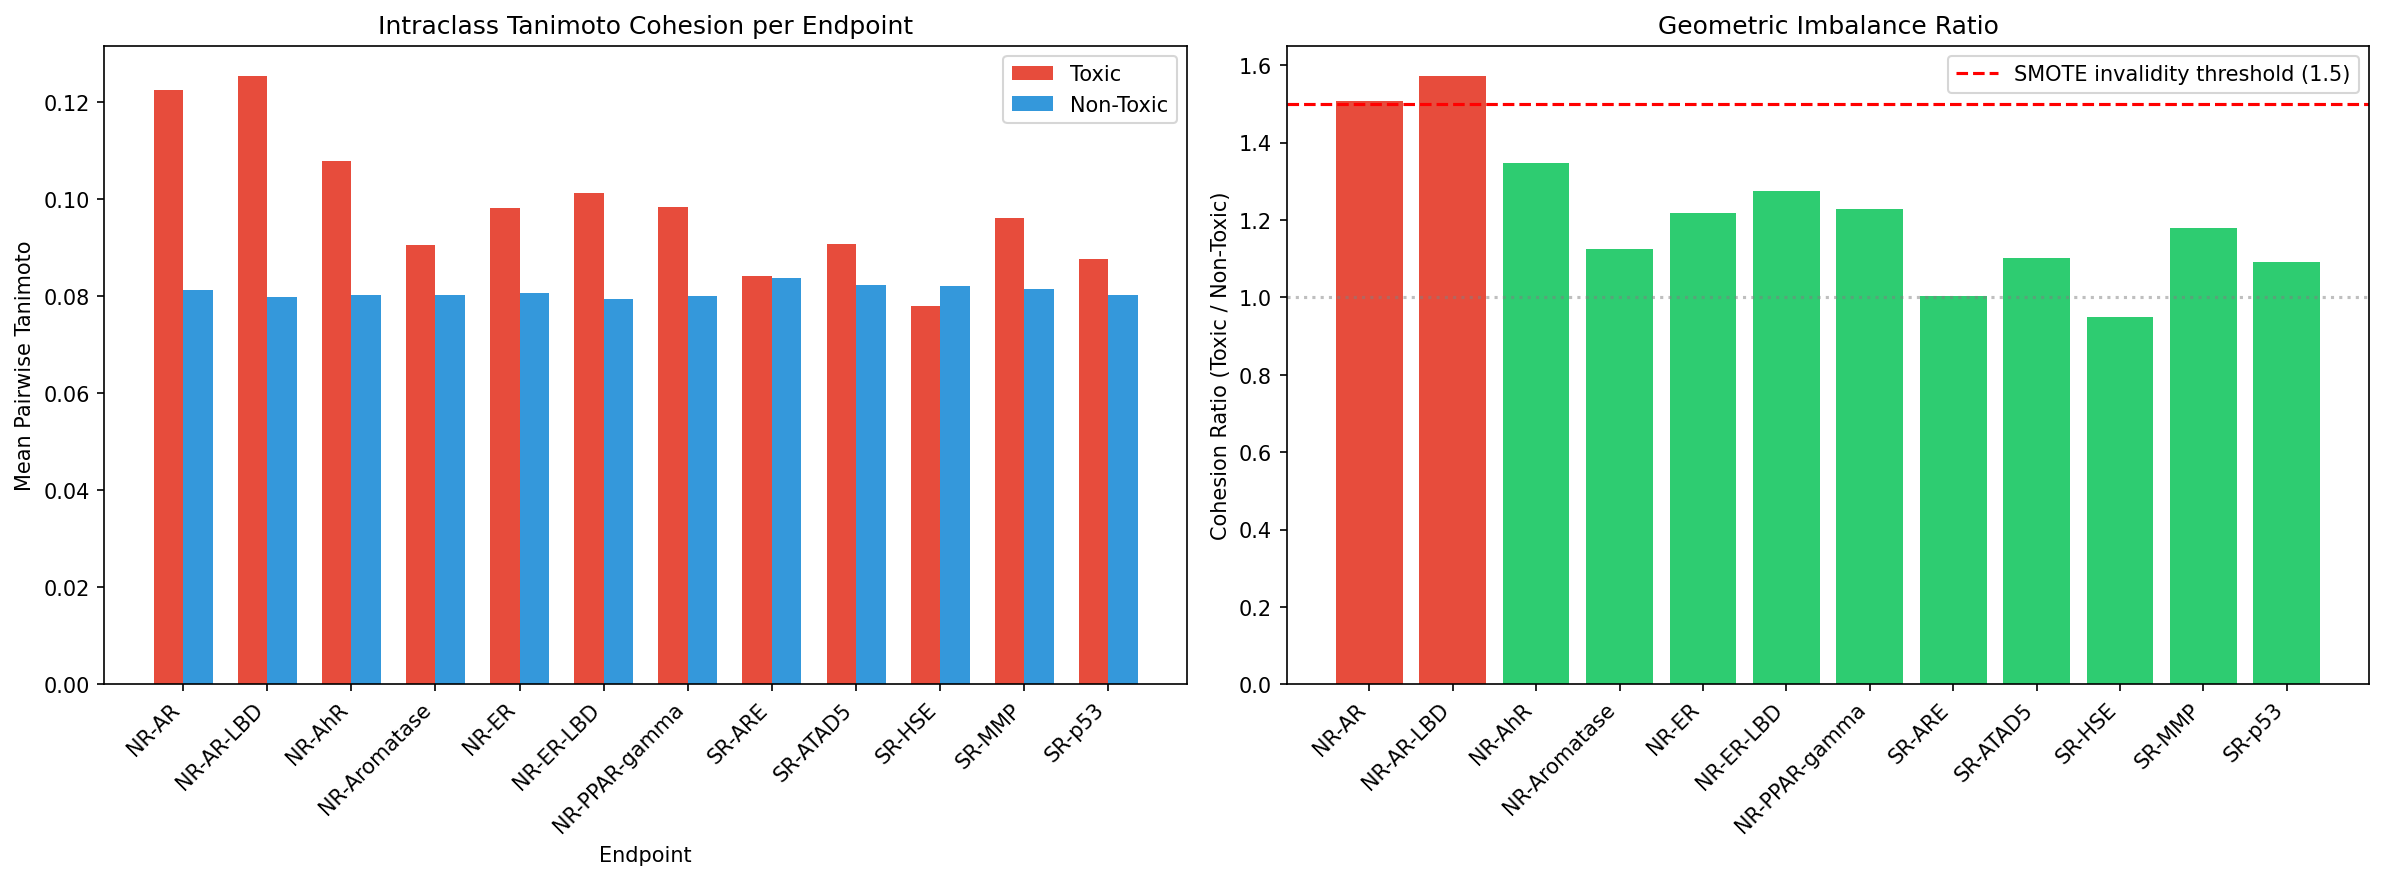
\includegraphics[width=3.0in]{02_geometric_imbalance.png}
\caption{Intraclass Tanimoto Cohesion analysis demonstrating the geometric imbalance of toxic compounds across the 12 Tox21 endpoints.}
\label{fig_geom_imb}
\end{figure}

\subsection{Prescriptive Efficacy}
When deployed as an end-to-end pipeline, ToxIntel successfully parsed known toxic inputs, cross-validated the SHAP attributions against structural alert databases, and retrieved ChEMBL bioisosteres. Through Pareto optimization, the system successfully identified candidate substitutions that strictly dominated the original molecule (i.e., reduced the probability of toxicity in the targeted endpoint without increasing the probability of toxicity across the remaining 11 endpoints). Mondrian Conformal Prediction successfully provided 90\% coverage guarantees, flagging candidates that drifted too far from the training distribution (Out-of-Distribution).

\section{Discussion}
The results demonstrate that treating molecular toxicity prediction strictly as a classification task ignores the geometric realities of chemical space and the ultimate needs of pharmaceutical design. While an AUPRC of 0.364 may appear low in standard machine learning contexts, in highly imbalanced biological datasets with inherent experimental noise, it represents a substantial predictive signal. Achieving this on a scaffold split guarantees that the model has learned the underlying biochemical mapping rather than memorizing dataset-specific structural similarities.

Furthermore, integrating Pareto optimization directly into the deep learning pipeline addresses a critical bottleneck in computer-aided drug design (CADD): the "whack-a-mole" problem, where fixing a toxic liability in the liver inadvertently creates a toxic liability in the heart. By enforcing a multi-endpoint Pareto front, ToxIntel guarantees global safety improvements. 

\subsection{Limitations}
There are limitations to the current implementation. First, the model relies on 2D topological fingerprints (ECFP4 \cite{ref5}) combined with basic physicochemical descriptors. This approach cannot capture complex 3D stereochemical interactions or conformational dynamics within the receptor binding pocket. Second, the Synthesizability Score (SAScore) used to filter bioisosteres is a heuristic estimate; true chemical synthesis planning requires rigorous retrosynthetic pathway analysis. Finally, Tox21 data is derived from \textit{in vitro} assays; thus, the model predicts the toxicity of the parent compound but does not account for the toxicity of \textit{in vivo} metabolites processed by hepatic CYP450 enzymes.

\section{Conclusion}
ToxIntel introduces a paradigm shift in computational toxicology, moving from reactive prediction to prescriptive structural optimization. By systematically quantifying geometric imbalance and applying a shared-backbone multi-task neural architecture with Focal Loss, we achieved a highly robust detection rate for rare toxic events. Crucially, by linking SHAP-based interpretability with Pareto-optimized bioisostere substitution and conformal prediction guarantees, ToxIntel provides actionable, structurally validated, and synthesizable solutions for drug designers. Future work will focus on integrating 3D geometric deep learning and comprehensive metabolic pathway prediction to further bridge the gap between \textit{in silico} models and clinical reality.

\section*{Acknowledgments}
% MISSING INFO: Add your acknowledgments here, e.g., thanking your professor.
This should be a simple paragraph before the References to thank those individuals and institutions who have supported your work on this article.

\begin{thebibliography}{1}
\bibliographystyle{IEEEtran}

\bibitem{ref1}
S. Barua, \textit{et al.}, ``Organ Toxicity ML: Oversampling and Hyperparameter Optimization for Imbalanced Chemical Datasets,'' [Online/Unpublished].

\bibitem{ref2}
Feitosa, \textit{et al.}, ``Cyto-Safe: Interpretable Machine Learning for Cytotoxicity Prediction Using SHAP,'' [Online/Unpublished].

\bibitem{ref3}
T.-Y. Lin, P. Goyal, R. Girshick, K. He, and P. Dollár, ``Focal Loss for Dense Object Detection,'' in \textit{Proc. IEEE Int. Conf. Comput. Vis. (ICCV)}, 2017.

\bibitem{ref4}
S. M. Lundberg and S.-I. Lee, ``A Unified Approach to Interpreting Model Predictions,'' in \textit{Adv. Neural Inf. Process. Syst. (NeurIPS)}, 2017.

\bibitem{ref5}
D. Rogers and M. Hahn, ``Extended-Connectivity Fingerprints,'' \textit{J. Chem. Inf. Model.}, 2010.

\bibitem{ref6}
Y. Zhang, \textit{et al.}, ``AI-Driven Drug Toxicity Prediction: Current Status and Open Problems in Clinical Interpretability,'' 2025.

\end{thebibliography}

\end{document}
